\documentclass[10pt]{beamer}
\usetheme{metropolis}
\usepackage{appendixnumberbeamer}
\usepackage[utf8]{inputenc}
\usepackage{lmodern}
\usepackage[french]{babel}
\usepackage{amsmath,amsthm,amssymb}
\usepackage{graphicx}
\usepackage{pgf,tikz}
\usepackage{tikzfmv}
\usepackage{mymath}
\usepackage{schemabloc}
\usepackage{caption}
\sbStyleBloc{thick}
\sbStyleLien{thick}
\usetikzlibrary{calc,tikzmark}
\usetikzlibrary{quotes,angles}
\usetikzlibrary{arrows.meta,bending,automata,positioning}
\usetikzlibrary{shapes.geometric}
\usetikzlibrary{shapes.misc}
\usetikzlibrary{babel}
\usetikzlibrary{decorations.text}
\usetikzlibrary{matrix}
\usepackage{pgfplots}
\pgfplotsset{compat=1.14} 
\usepackage{array,multirow,makecell}
\usepackage{hhline}
\newcolumntype{K}[1]{>{\centering\arraybackslash}p{#1}}
\newcolumntype{M}[1]{>{\centering\arraybackslash}m{#1}}
\newcolumntype{N}{@{}m{0pt}@{}}
%\usepackage[dvipsnames]{xcolor}

\begin{document}

%%%%%%%%%%%%%%%%%%%%%%%%%%%%%%%%%%%%%%%%%%%%%%%%%%%%%%%%%%%%%%%%%%%%%%%%%%%%%%%%%%
\begin{frame}
    \frametitle{Réponses temporelles du 2nd ordre}
    \newcommand{\mysize}{\footnotesize}
\resizebox{\textwidth}{!}{
        \begin{tabular}{M{2.75cm}M{5.25cm}M{5.25cm}M{5.25cm}}%
        \hhline{====}
             Réponse   & Régime apérodique        ($\xi>1$)  & Régime critique ($\xi=1$) & 
                         Régime pseudo-périodique ($0<\xi<1$) \\[0em]
        \hline
        Réponse impulsionnelle & 
            \resizebox{0.9\linewidth}{!}{\begin{tikzpicture}
    \begin{axis}
    [   legend style={draw=none},
        axis line style = thick,
        xmin=0,
        xmax=12,
        ymin=0,
        ymax=0.3,
        xlabel={$t$},
        ylabel={$s(t)$},
        label style={font=\Large},
        grid=both,
        grid style={line width=.4pt, draw=black},
        major grid style={line width=.4pt,draw=black},
    ]
    \addplot[signalb,domain=0:12] {(1/(3.73-0.26))*exp(-x/3.73)-exp(-x/0.26)};
    \end{axis}
\end{tikzpicture}
} 
            {\mysize $$ s(t)=\dfrac{1}{\tau_1-\tau_2}\left(e^{-\frac{t}{\tau_1}}-e^{-\frac{t}{\tau_2}}\right)$$} &  
            \resizebox{0.9\linewidth}{!}{    \begin{tikzpicture}
        \begin{axis}[
        legend style={draw=none},
        axis line style = thick,
        xmin=0,
        xmax=10,
        ymin=0,
        ymax=0.4,
        xlabel={$t$},
        ylabel={$s(t)$},
        label style={font=\Large},
        ]
            \addplot [thick,color=blue,domain=0:11.5, samples=101,unbounded coords=jump]{x*exp(-x)};
        \end{axis}
    \end{tikzpicture}
} 
            {\mysize $$s(t)=\dfrac{t}{\tau^2}e^{-\frac{t}{\tau}}$$} &  
            \resizebox{0.9\linewidth}{!}{\tikzsetnextfilename{2nd_rep_1_3_ext}
\begin{tikzpicture}
    \begin{axis}
    [   legend style={draw=none},
        axis line style = thick,
        xmin=0,
        xmax=12,
        ymin=-0.6,
        ymax=1.2,
        xlabel={$t$},
        ylabel={$s(t)$},
        label style={font=\Large},
        grid=both,
        grid style={line width=.4pt, draw=black},
        major grid style={line width=.4pt,draw=black},
    ]
    \def\a{0.3}            
    \def\b{0.91}           
    \def\w{0.953939201417} 
    \addplot[signalb,domain=0:12] {(\w/\b)*exp(-\a*x)*sin(deg(x)*\w)};
    \end{axis}
\end{tikzpicture}
} 
            {\mysize $$s(t)=\dfrac{\omega_d}{1-\xi^2}e^{-\xi\omega_0 t}\sin{\omega_d t}$$}\\[0em]
        \hline
        Réponse indicielle &  
            \resizebox{0.9\linewidth}{!}{\tikzsetnextfilename{2nd_rep_2_1_ext}
\begin{tikzpicture}
    \def\tu{2.0}
    \def\td{1.0}
    \begin{axis}
    [   legend style={draw=none},
        axis line style = thick,
        xmin=0,
        xmax=10,
        ymin=0,
        ymax=1.2,
        xlabel={$t$},
        ylabel={$s(t)$},
        label style={font=\Large},
    ]
    \addplot[very thick,color=blue,domain=0:11.5, samples=101]
    {1+(1/(3.73-0.26))*(0.26*exp(-x/0.26)-3.73*exp(-x/3.73))};
    \end{axis}
\end{tikzpicture}
} 
            {\mysize $$s(t)=1+\dfrac{1}{\tau_1-\tau_2}\left(\tau_2e^{-\frac{t}{\tau_2}}-\tau_1e^{-\frac{t}{\tau_1}}\right)$$} &  
            \resizebox{0.9\linewidth}{!}{\begin{tikzpicture}
    \begin{axis}
    [   legend style={draw=none},
        axis line style = thick,
        xmin=0,
        xmax=10,
        ymin=0,
        ymax=1.2,
        xlabel={$t$},
        ylabel={$s(t)$},
        label style={font=\Large},
        grid=both,
        grid style={line width=.4pt, draw=black},
        major grid style={line width=.4pt,draw=black},
    ]
    \addplot[signalb,domain=0:10]  {1-exp(-x)-x*exp(-x)};
    \end{axis}
\end{tikzpicture}
} 
            {\mysize $$s(t)=1-e^{-\frac{t}{\tau}}-\dfrac{t}{\tau}e^{-\frac{t}{\tau}}$$ } &  
            \resizebox{0.9\linewidth}{!}{\tikzsetnextfilename{2nd_rep_2_3_ext}
\begin{tikzpicture}
\begin{axis}
[   
    legend style={draw=none},
    axis line style = thick,
    xmin=0,
    xmax=12,
    ymin=0,
    ymax=1.5,
    xlabel={$t$},
    ylabel={$s(t)$},
    label style={font=\Large},
    grid=both,
    grid style={line width=.4pt, draw=black},
    major grid style={line width=.4pt,draw=black},
]
\def\a{0.3}            
\def\b{0.91}           
\def\w{0.954} 
\def\p{1.266}  
\addplot[signalb,domain=0:12] {1-((1./\w)*exp(-\a*x)*sin(deg(x)*\w+deg(\p)))};
\end{axis}
\end{tikzpicture}
} 
            {\mysize $$s(t) = 1 - \dfrac{e^{-\xi\omega_0 t}}{\sqrt{1-\xi^2}}\sin{(\omega_d t+\phi)}$$}\\[0em]
        \hhline{====}
        \end{tabular}
}


\end{frame}
%%%%%%%%%%%%%%%%%%%%%%%%%%%%%%%%%%%%%%%%%%%%%%%%%%%%%%%%%%%%%%%%%%%%%%%%%%%%%%%%%%
\begin{frame}[fragile]
    \frametitle{Temps de réponse à 5\%}
\begin{center}
    \begin{tikzpicture}                                                                                          
\pgfmathsetmacro{\a}{0.2}             % amortissement xi                                                 
\pgfmathsetmacro{\b}{0.96}            % 1-xi^2                                                           
\pgfmathsetmacro{\w}{0.979795897113}  % w_d=w_0 sqrt(1-xi^2)                                             
\pgfmathsetmacro{\p}{1.369438406}     % phi =arctan(xi/1-xi^2)                                           
\begin{axis}[                                                                                            
            axis line style = thick,                                                                             
            %height=8cm,                                                                                         
            %width=12cm,                                                                                         
            axis x line=center,                                                                                  
            axis y line=center,                                                                                  
            xmin=-0.1,                                                                                           
            xmax=20,                                                                                             
            ymin=-0.1,                                                                                           
            ymax=1.6,                                                                                            
            xlabel={$t$},                                                                                        
            ylabel={$s(t)$},                                                                                     
            xlabel style={below right},                                                                          
            ylabel style={left},                                                                                 
            xticklabels={2,\textcolor{red}{$t_1$},10,\textcolor{blue}{$t_2$}},                                   
            xtick={2,5.29,10,13.74},                                                                             
            yticklabels={0,$KE_0$,2},                                                                            
            ytick={0.001,1,2}
]
    \addplot[thick,color=blue,domain=0:20, samples=101,unbounded coords=jump]{1-((1./\w)*exp(-\a*x)*sin(deg(x)*\w+deg(\p)))};
    \addplot[thick,domain=0:20, samples=101,unbounded coords=jump]{1};
    \addplot[dotted,domain=0:20, samples=101,unbounded coords=jump]{1.05};
    \addplot[dotted,domain=0:20, samples=101,unbounded coords=jump]{0.95};
    \def\a{0.5}
    \def\b{0.75}
    \def\w{0.866025403784}                                                                                   
    \def\p{1.0471975512}
    \addplot [thick,domain=0:20, color=red,samples=101,unbounded coords=jump]{1-((1./\w)*exp(-\a*x)*sin(deg(x)*\w+deg(\p)))};
    \draw[blue,thick] (axis cs:13.74,0) -- (axis cs:13.74,2);
    \draw[red,thick] (axis cs:5.29,0) -- (axis cs:5.29,2);
    \end{axis}                                                                                               
\end{tikzpicture}                                                                                            

\end{center}
\end{frame}
%%%%%%%%%%%%%%%%%%%%%%%%%%%%%%%%%%%%%%%%%%%%%%%%%%%%%%%%%%%%%%%%%%%%%%%%%%%%%%%%%%
\begin{frame}
    \frametitle{Relation temps de réponse-amortissement}
    \centering
    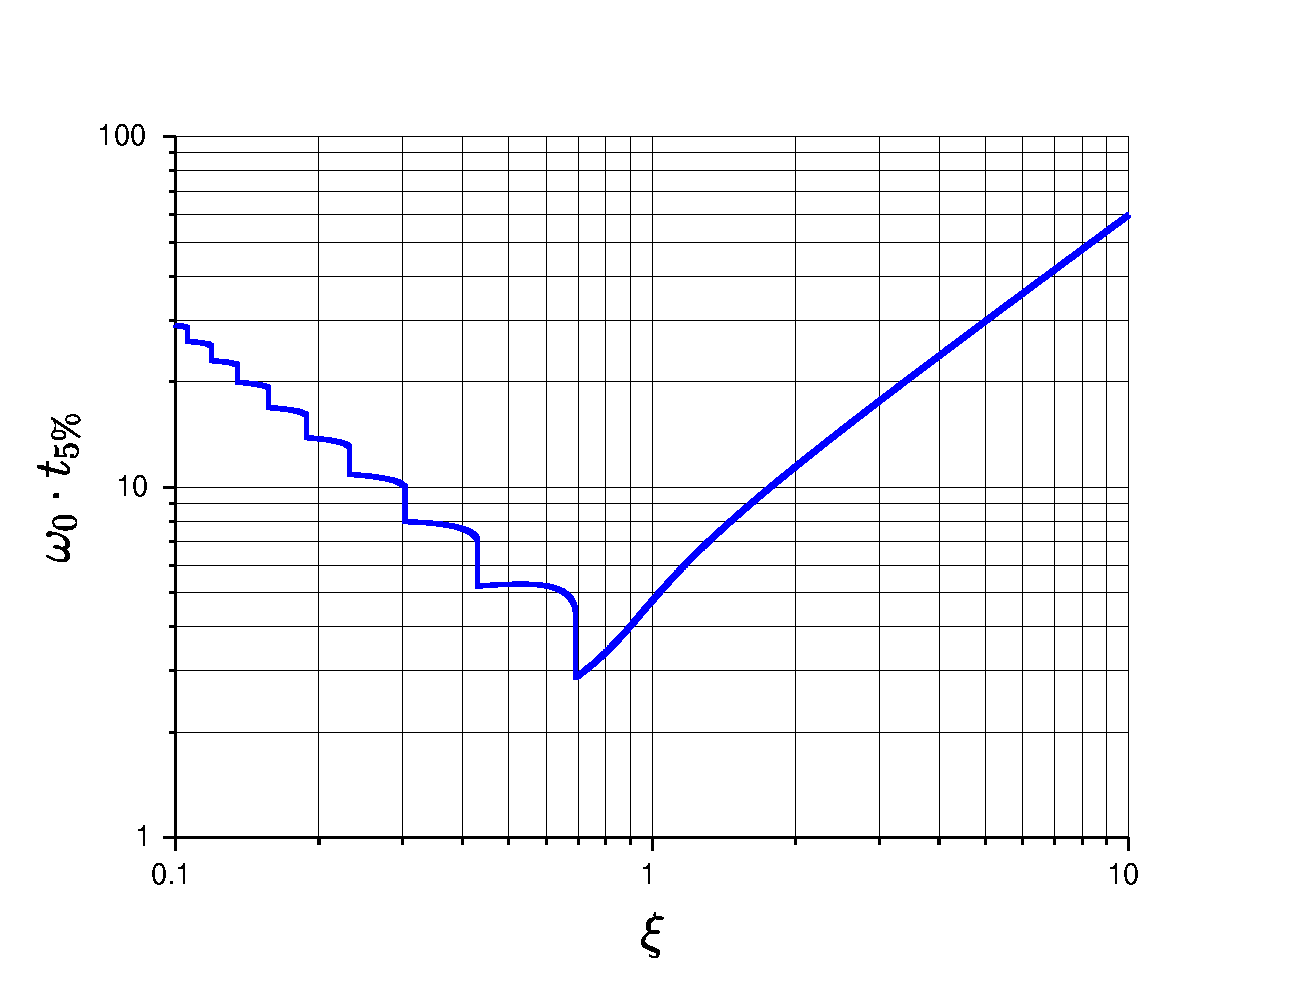
\includegraphics[width=0.7\textwidth]{fig/fig_temps_de_reduit.eps}
\end{frame}
%%%%%%%%%%%%%%%%%%%%%%%%%%%%%%%%%%%%%%%%%%%%%%%%%%%%%%%%%%%%%%%%%%%%%%%%%%%%%%%%%%
\begin{frame}[fragile]
    \frametitle{Dépassement}
\begin{center}
        \begin{tikzpicture}                                                                                          
        \pgfmathsetmacro{\a}{0.2}             % amortissement xi                                                 
        \pgfmathsetmacro{\b}{0.96}            % 1-xi^2                                                           
        \pgfmathsetmacro{\w}{0.979795897113}  % w_d=w_0 sqrt(1-xi^2)                                             
        \pgfmathsetmacro{\p}{1.369438406}     % phi =arctan(xi/1-xi^2)                                           
        \pgfmathsetmacro{\tu}{3.206374575405548}    % t1 =                                                       
        \pgfmathsetmacro{\td}{6.4127491508093204}   % t2 = 2*t1                                                  
        \pgfmathsetmacro{\ttt}{9.619123726213981}    % t3 = 3*t1                                                 
        \pgfmathsetmacro{\tq}{12.82549830161864}    % t4 = 4*t1                                                  
        \pgfmathsetmacro{\du}{1.526620599330303}     % dépassement d1                                            
        \pgfmathsetmacro{\dd}{0.72267074436099255}     % dépassement d2                                          
        \pgfmathsetmacro{\dt}{1.146047298816441}     % dépassement d3                                            
        \pgfmathsetmacro{\dq}{0.92308848396671406}     % dépassement d4                                          
                                                                                                                 
        %>>> 1+np.exp(-0.2*np.pi/np.sqrt((1-0.2*0.2)))+1                                                         
        %>>> 1-np.exp(-2*0.2*np.pi/np.sqrt((1-0.2*0.2)))+1                                                       
        %>>> 1+np.exp(-3*0.2*np.pi/np.sqrt((1-0.2*0.2)))+1                                                       
        %>>> 1-np.exp(-4*0.2*np.pi/np.sqrt((1-0.2*0.2)))+1                                                       
        %1.526620599330303                                                                                       
        %0.72267074436099255                                                                                     
        %1.146047298816441                                                                                       
        %0.92308848396671406                                                                                     
                                                                                                                 
        \begin{axis}[                                                                                            
        %ticks=none,                                                                                             
        axis line style = thick,                                                                                 
        %height=9cm,                                                                                             
        %width=12cm,                                                                                             
        axis x line=center,                                                                                      
        axis y line=center,                                                                                      
        xmin=-0.1,                                                                                               
        xmax=20,                                                                                                 
        ymin=-0.1,                                                                                               
        ymax=2.2,                                                                                                
        xlabel={$t$},                                                                                            
        ylabel={$s(t)$},                                                                                         
        xlabel style={below right},                                                                              
        ylabel style={left},                                                                                     
        xticklabels={$t_1$,$t_2$,$t_3$,$t_4$},                                                                   
        xtick={\tu,\td,\ttt,\tq},                                                                                
        yticklabels={0,$KE_0$,$2KE_0$},                                                                          
        ytick={0.001,1,2}                                                                                        
        ]                                                                                                        
        \addplot [thick,color=blue,domain=0:20, samples=101,unbounded coords=jump]{1-((1./\w)*exp(-\a*x)*sin(deg(x)*\w+deg(\p)))};                                                                                                
        \addplot [thick,dotted,domain=0:20, samples=101,unbounded coords=jump]{1+exp(-\a*x)};                    
        \addplot [thick,dotted,domain=0:20, samples=101,unbounded coords=jump]{1-exp(-\a*x)};                    
        \addplot [thick,domain=0:20, samples=101,unbounded coords=jump]{1};                                      
            \draw [ultra thick, red] (axis cs:\tu,1)  -- (axis cs:\tu,\du) node[above] {$D_1$};                  
            \draw [ultra thick, blue] (axis cs:\td,1)  -- (axis cs:\td,\dd) node[below] {$D_2$};                 
            \draw [ultra thick, green] (axis cs:\ttt,1) -- (axis cs:\ttt,\dt) node[above] {$D_3$};               
            \draw [ultra thick, black] (axis cs:\tq,1)  -- (axis cs:\tq,\dq) node[below] {$D_4$};
            \draw (axis cs:\tu,0) -- (axis cs:\tu,0.1);
            \draw (axis cs:\td,0) -- (axis cs:\td,0.1);
        \end{axis}
    \end{tikzpicture}

\end{center}                                                                                                     
\end{frame}           
%%%%%%%%%%%%%%%%%%%%%%%%%%%%%%%%%%%%%%%%%%%%%%%%%%%%%%%%%%%%%%%%%%%%%%%%%%%%%%%%%%
\begin{frame}[fragile]
    \frametitle{Relation dépassement-amortissement}
\begin{center}
\begin{tikzpicture}
    \pgfplotsset{signaltmp/.style={signaln,domain=0.0001:1,
                              unbounded coords=jump}
                }
    \pgfmathsetmacro{\pi}{3.141592653589793}     % dépassement d4 
    \begin{axis}
    [   xmode=log,
        ymode=log,
        width=0.65\textwidth,
        axis line style = thick,
        xmin=0.01,
        xmax=1,
        ymin=0.01,
        ymax=1.0,
        xlabel={$\xi$},
        ylabel={$D_k$},
        label style={font=\Large},
        grid=both,
        grid style={line width=.4pt, draw=black},
        major grid style={line width=.4pt,draw=black},
        legend style={draw=none,font=\normalsize},
        legend pos=outer north east,
        label style={font=\Large},
        legend cell align={left},
    ]
    \addplot[signaltmp,vtcol1] {exp(-(x*\pi)/(sqrt(1-x*x)))};
    \addplot[signaltmp,vtcol2] {exp(-(2*x*\pi)/(sqrt(1-x*x)))};
    \addplot[signaltmp,vtcol3] {exp(-(3*x*\pi)/(sqrt(1-x*x)))};
    \addplot[signaltmp,vtcol4] {exp(-(4*x*\pi)/(sqrt(1-x*x)))};
    \legend{$k=1$,$k=2$,$k=3$,$k=4$}
    \end{axis}
\end{tikzpicture}


\end{center}
\end{frame}
%%%%%%%%%%%%%%%%%%%%%%%%%%%%%%%%%%%%%%%%%%%%%%%%%%%%%%%%%%%%%%%%%%%%%%%%%%%%%%%%%%

\end{document}



